\begin{center}
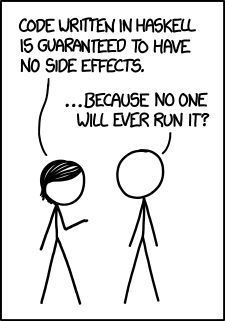
\includegraphics[width=0.3\textwidth]{haskell-1312.png}
\end{center}
\begin{center}
\url{http://xkcd.com/1312/}
\end{center}

\section{Über die Programmiersprache}
Die Einleitung in \cite{lyahfgg} sagt folgendes über Haskell.

\begin{itemize}
  \item
Haskell ist eine \emph{rein funktionale} Programmiersprache.
In einer \emph{imperativen} Programmiersprache gibt man dem Computer eine Folge
von Aufgaben, welche dann ausgeführt werden.  Dazu gibt es Strukturen, die den
Ablauf steuern, wie beispielsweise \texttt{for} und \texttt{while}.

Anders hingegen in einer funktionalen Programmiersprache. Man sagt dem Computer
nicht, was er tun soll. Stattdessen sagt man ihm eher, was die Sachen sind.
Zum Beispiel, kann man dem Computer sagen, dass die Fakultät einer Zahl das
Produkt aller Zahlen von $1$ bis zu dieser Zahl ist.
Dies wird als eine, häufig rekursive, Funktion ausgedrückt.

Beim funktionalen Programmieren kann man keine Werte von Variablen verändern.
In einer rein funktionalen Programmiersprache hat eine Funktion keine
Seiteneffekte. Das einzige was eine Funktion tun kann, ist eine Berechnung,
basierend auf ihren Eingaben. Das scheint eine Einschränkung zu sein, aber in
der Tat hat dies einige positive Konsequenzen. Beispielsweise liefert eine
Funktion bei gleichen Eingaben, unabhängig von der Umgebung, immer den gleichen
Rückgabe Wert. Diese Eigenschaft heißt \emph{Referentielle Transparenz}.

  \item
Haskell ist \emph{lazy}.
Das bedeutet, dass Haskell Funktionen nicht auswertet, solange das Ergebnis
nicht benötigt wird. Dies wird durch Referentielle Transparenz ermöglicht.
Haskell bemüht sich, die Auswertungen von Ausdrücken so lange wie möglich zu
vermeiden.
Es wird damit auch ermöglicht scheinbar unendliche Datenstrukturen zu
verwenden, da nur Teile, also so weit wie nötig, evaluiert werden.

  \item
Haskell ist \emph{statisch Typisiert}.
Das bedeutet, dass der Computer bereits zur Compilezeit weiß, welcher Teil eine
Zahl ist und was eine Funktion ist, die aus einer Liste von Zahlen einen String
macht, usw. Das bedeutet, dass viele Fehler bereits während des Compilierens
erkannt werden können.

Zusätzlich ist Haskell auch noch sehr gut darin, Typen zu inferieren. Das
bedeutet, das man meist nicht extra angeben muss, welchen Typ jeder Teil im
Code hat. Beispielsweise erkennt Haskell aus \texttt{a = 4 + 5} dass
\texttt{a} eine Zahl sein muss.
Damit ist es auch leichter, allgemeineren Code zu schreiben, der an vielen
Stellen anwendbar ist.

  \item
Haskell ist \emph{elegant und präzise}.
Da Haskell viele Konzepte höherer Programmiersprachen nutzt, sind in Haskell
geschriebene Programme meist kürzer als ein vergleichbares imperatives. Und
kürzere Programme sind einfacher zu Warten und enthalten weniger Fehler.
\end{itemize}

Die Haskell Entwicklung begann 1987, als sich eine Gruppe von Wissenschaftlern
zusammengetan hat, um eine Programmiersprache zu entwickeln, die ihren
Ansprüchen genügt. Der \emph{Haskell Report}, welcher die erste stabile Version
beschreibt, wurde 1999 publiziert (überarbeitet Version: \cite{haskell98}).
Der aktuelle Standard wird beschrieben in \cite{haskell2010}.

Gute Bücher zum Einstieg in Haskell sind beispielsweiße \cite{Hutton} und
\cite{lyahfgg}.
Basierend auf \cite{Hutton} gibt es von Erik Meijer auch eine ausführliche
Video Reihe, die leicht im Internet zu finden ist.
Zum Buch \cite{lyahfgg} gibt es ebenfalls im Internet eine vollständige HTML
Variante\footnote{\url{http://learnyouahaskell.com/}}.

\iffalse
Es ist auch die Seite \url{http://en.wikibooks.org/wiki/Haskell} sehr
empfehlenswert.
\fi

Eine ausführliche Übersicht über Tutorials bietet die Seite
\url{http://www.haskell.org/haskellwiki/Tutorials}.

Eine Liste an Büchern bietet \url{http://www.haskell.org/haskellwiki/Books}.

\section{Ausführen von Haskell Programmen}

Haskell kann jederzeit interpretiert oder compiliert werden. Mit dem
Interpreter \texttt{ghci} oder \texttt{hugs} kann man einfach Programme oder
Code-Schnipsel testen.
Alternativ erhält man durch compilieren mit \texttt{ghc} ausführbare Dateien,
welche dank recht umfangreicher Optimierung performanter sind. Für eine
ausführlichere Optimierung gibt es den Compiler Parameter \texttt{-O}. Noch
mehr Optimierung verspricht \texttt{-O2}, wobei das compilieren damit
nochmals deutlich länger dauert.

Die Compileroption \texttt{-threaded} bereitet die ausführbare Datei darauf
vor, parallel ausgeführt zu werden. Zusätzlich muss man beim ausführen dann
noch die Parameter \texttt{-RTS -N4} mitgeben, wobei die $4$ die Anzahl der
Prozessorkerne angibt, die genutzt werden sollen.

\section{Installieren von Haskell Paketen}
Zum installieren gibt es das Konsolenwerkzeug
\texttt{cabal}\footnote{\url{http://www.haskell.org/cabal/download.html}} für
Windows und Unix Systeme.
Durch ausführen von
\begin{lstlisting}[language=bash 
                  ,numbers=none
                  ,backgroundcolor=\color{lightgray}]
cabal update
\end{lstlisting}
holt sich dieses, aktuelle Paketlisten von
\url{https://hackage.haskell.org/}. Danach kann man mittels
\begin{lstlisting}[language=bash
                  ,numbers=none
                  ,backgroundcolor=\color{lightgray}]
cabal install PAKETNAME
\end{lstlisting}
Pakete aus der umfangreichem Bibliothek installieren.
Dabei löst \texttt{cabal} selbstständig die Abhängigkeiten auf.

\section{Entwicklung von Haskell-Code}
Für Haskell gibt es eine umfangreiche Auswahl an Programmen, die einem bei der
Entwicklung von Haskell Bibliotheken und Programmen helfen. Hier sollen die
erwähnt werden, die für dieses Projekt genutzt wurden.

\subsection{Testing: \texttt{hspec}}
\begin{quote}
  Hspec is roughly based on the Ruby library RSpec. However, Hspec is just a
  framework for running HUnit and QuickCheck tests. Compared to other options,
  it provides a much nicer syntax that makes tests very easy to
  read.\footnote{\url{https://hackage.haskell.org/package/hspec}}
\end{quote}
Hspec ermöglicht es einfach tests zu schreiben, deren Quellcode leicht
verständlich ist und eine konkrete Aussage darüber trifft, was die getestete
Funktion tuen sollte.

Ein einfaches und selbsterklärendes
Beispiel\footnote{\url{http://hspec.github.io/}} ist
\begin{hcode}
-- Datei Spec.hs
import Test.Hspec
import Test.QuickCheck
import Control.Exception (evaluate)

main :: IO ()
main = hspec $ do
  describe "Prelude.head" $ do
    it "returns the first element of a list" $ do
      head [23 ..] `shouldBe` (23 :: Int)

    it "returns the first element of an *arbitrary* list" $
      property $ \x xs -> head (x:xs) == (x :: Int)

    it "throws an exception if used with an empty list" $ do
      evaluate (head []) `shouldThrow` anyException
\end{hcode}
Ein Ausführen, durch beispielsweise \texttt{runhaskell Spec.hs},liefert die folgende
Konsolenausgabe
\begin{lstlisting}[language=bash 
                  ,numbers=none
                  ,backgroundcolor=\color{lightgray}]
Prelude.head
  - returns the first element of a list
  - returns the first element of an *arbitrary* list
  - throws an exception if used with an empty list

Finished in 0.0028 seconds
3 examples, 0 failures
\end{lstlisting}

\subsection{Benchmarking: \texttt{criterion}}
\begin{quote}
  This library provides a powerful but simple way to measure software
  performance. It provides both a framework for executing and analysing
  benchmarks and a set of driver functions that makes it easy to build and run
  benchmarks, and to analyse their
  results.\footnote{\url{https://hackage.haskell.org/package/criterion}}
\end{quote}

\subsection{Zusammenfügen: \texttt{cabal}}
\begin{quote}
  The Haskell Common Architecture for Building Applications and Libraries: a
  framework defining a common interface for authors to more easily build their
  Haskell applications in a portable way.

  The Haskell Cabal is part of a larger infrastructure for distributing,
  organizing, and cataloging Haskell libraries and
  tools.\footnote{\url{https://hackage.haskell.org/package/Cabal}}
\end{quote}
Weitere Quellen:
\begin{itemize}
  \item \url{http://www.haskell.org/haskellwiki/How_to_write_a_Haskell_program}
\end{itemize}

\subsection{Dokumentation: \texttt{haddock}}
\begin{quote}
  Haddock is a tool for automatically generating documentation from annotated
  Haskell source code.\footnote{\url{http://www.haskell.org/haddock/}}
\end{quote}

\section{Das Haskell Typensystem}
In Haskell weiß jeder Ausdruck bereits zur Compilezeit, welchen Typ er hat. So
werden Fehler wie das Diviedieren eines Boolean durch eine Zahl bereits während
des Compilierens aufgedeckt und müssen nicht durch Glück wärend des Ausführens
gefunden werden. Gekennzeichnet werden Typenangaben in Haskell durch ħ::ħ als
Infix-Operator. Die folgende Aussage bedeutet, dass eine Variable ħcountħ vom Typ
ħIntħ ist.
\begin{hcode}
count :: Int
\end{hcode}
Da es in Haskell Higher-Order Funktionen gibt haben natürlich auch Funktionen
einen Typ. Beispielsweise hat die Funktion ħheadħ, welche zu einer Liste das
erste Element wiedergibt, den Typ:
\begin{hcode}
head :: [a] -> a
\end{hcode}
Zu bemerken ist hier, dass für die Funktion nicht vorgegeben ist, von welchem
Typ die Elemente der Liste sind. So kann die Typen Variable ħaħ für jeden Typen
stehen, also funktioniert die Funktion beispielsweise auf Listen von Zahlen.
Ebenso funktioniert sie aber für Strings, welche in Haskell als Listen von
Zeichen implementiert sind.

Weiter gibt es Typen Klassen, welche beispielsweise den Interfaces von Java
ähneln.  Eine Klasse beschreibt dabei ein Verhalten von Typen. Um zu sagen,
dass ein Typ das Verhalten einer Klasse hat, muss man für diesen eine Instanz
dieser Klasse implementieren.
Dazu besteht jede Klasse aus einer vorgegebenen Liste von Funktionen, welche
implementiert werden müssen. Ein gutes Beispiel hierfür ist ħEqħ, welches als
einzige Funktion den Operator ħ(==)ħ\footnote{Die Schreibweise mit den Klammern
dient dazu, Infix-Operatoren zu definieren.} enthält. Also muss man sagen,
welche Werte oder Konstruktorterme des Typs gleich sein sollen.

Die Funktion ħ(==)ħ selbst hat den Typ
\begin{hcode}
(==) :: (Eq a) => a -> a -> Bool
\end{hcode}
wobei das ħ=>ħ ein Zeichen ist, das eine Typen Klassen Restriktion beschreibt.
Hier darf also die Typen Variable ħaħ nicht durch alle Typen ersetzt werden,
sondern nur durch die, die eine Instanz ħEqħ haben. Also können wir Werte auf
Gleichheit nur dann Prüfen, wenn wir eine Instanz ħEqħ haben. Freie Datentypen
werden, sofern nicht extra eine Instanz von ħEqħ erzeugt wurde, auf
strukturelle Gleichheit geprüft.

Eine umfangreiche Liste an wichtigen Typen Klassen sowie eine ausführlichere
Erklärung das Haskell Typensystems findet man beispielsweise in \cite{lyahfgg}
im zweiten Kapitel.

\section{Pragmas} %TODO: oder Paradigmen?
Pragmas\footnote{\url{https://www.haskell.org/ghc/docs/7.0.4/html/users_guide/pragmas.html}}
bieten in Haskell die Möglichkeit, für den Compiler bestimmte Commandos in den
Quellcode zu integrieren. Diese beeinflussen meist nicht die Bedeutung des
Codes sondern haben eher Einfluss auf Effizienz des generierten Programms. Auch
können damit Haskell Erweiterungen aktiviert werden.

Ein (Sprach) Pragma im Code ist berandet durch ħ{-# ... #-}ħ und ein Beispiel
dafür wäre
\begin{hcode}
{-# LANGUAGE CPP #-}
{-# LANGUAGE TemplateHaskell #-}
\end{hcode}
Dadurch werden die (Sprach-) Erweiterungen \texttt{CPP} und
\texttt{TemplateHaskell} aktiviert. Die erste Erweiterung ermöglicht es durch
die Befehle \texttt{\#if 1} bzw. \texttt{\#if 0}, \texttt{\#else} und
\texttt{\#endif} analog zu \texttt{\slash{}iftrue} und
\texttt{\slash{}iffalse} im \LaTeX{} mehrere Zeilen im Quellcode zu
deaktivieren bzw. schnell zwischen alternativen Implementierungen umzuschalten.

Die \texttt{TemplateHaskell} ermöglicht es, zusammen mit \texttt{QuasiQuotes}
Haskell Funktionen bereits zur Compilezeit auszuführen. Damit lässt sich
dynamisch Code erzeugen oder man kann auch Rechenaufgaben in die Compilezeit
verlagern.

Es gibt noch diverse andere Arten von Pragmas, die beispielsweise:
\begin{itemize}
  \item \texttt{OPTIONS\_GHC} Pragmas bieten eine Möglichkeit, dem Compiler
    direkt Compileparameter zu übergeben und
  \item ħINLINEħ Pragmas werden in der Form
    ħ{-# INLINE funktionsname #-}ħ einer Funktion direkt vorangestellt und 
    und geben dem Compiler die Anweisung, den Inhalt der Funktion anstelle des
    Funktionsaufrufs bei einer Benutzung zu setzen. Wird innerhalb eines
    Programms eine Funktion, nennen wir sie ħfooħ benutzt, so setzt der
    Compiler an diese Stelle lediglich eine Referenz auf die Funktion ħfooħ,
    deren eigentliche Definition an irgendeiner anderen Stelle gespeichert wird.
    Das ħINLINEħ-Pragma fordert nun den Compiler auf, die gesamte Definition 
    von ħfooħ statt einer Referenz zu setzen. Dies spart
    bei der Ausführung -- gerade wenn die Funktion häufig mit wechselnden
    Argumenten aufgerufen wird, wie
    beispielsweise eine Addition -- Zeit, da das Programm die aktuelle Position
    der Ausführung nicht verlassen muss. Dies geht jedoch auf Kosten einer gewissen
    Lazyness. Nehmen wir an, ħfooħ hätte die Deklaration ħfoo :: a -> aħ und wir
    würden in einem fiktiven Programm sehr oft ħfoo ħ$x$ mit dem selben Argument
    $x$ aufrufen, so würde ohne ħINLINEħ Haskell lediglich \emph{einmal}
    ħfoo ħ$x$ berechnen und die anderen Aufrufe durch das Ergebnis ersetzen.
    Durch ħINLINEħ wird ħfooħ sofort durch seinen Inhalt ersetzt, wodurch 
    \emph{alle} ħfoo ħ$x$ separat berechnet werden. 
\end{itemize}
